\begin{table}[h!]
	\centering
	\small
	\scalebox{0.78}{
		\begin{tabular}{|c|c|c|c|c|c|}
			\hline 
			No & \makecell{Candidate\\biomarker}& Formula & \makecell{Chemical\\group} &Presence in Food & Reference\\ 
			\hline 
			1&Hordenine& C\textsubscript{10}H\textsubscript{15}NO &alkaloid&\makecell{germinating barley,\\ beer and other plants}&\cite{Gurdeniz2016}\\ 
			\hline
			4&Hordatine A&C\textsubscript{28}H\textsubscript{38}N\textsubscript{8}O\textsubscript{5}&alkaloid&\makecell{only reported\\in barley}&\makecell{FoodDB\\(002330)}\\ 
			\hline 
			4&Hordatine B&C\textsubscript{29}H\textsubscript{40}N\textsubscript{8}O\textsubscript{5}&alkaloid&\makecell{only reported\\in barley}&\makecell{FoodDB\\(002328)}\\ 
			\hline 
			2&\makecell{Distichonic\\acid A}&C\textsubscript{10}H\textsubscript{18}N\textsubscript{2}O\textsubscript{8}&\makecell{gamma amino acids\\ and derivatives}&\makecell{only reported\\in barley}&\makecell{FoodDB\\(18164)}\\
			\hline 
			3&\makecell{Distichonic\\acid B}&C\textsubscript{10}H\textsubscript{18}N\textsubscript{2}O\textsubscript{8}&\makecell{gamma amino acids\\ and derivatives}&\makecell{only reported\\in barley}&\makecell{FoodDB\\(018165)}\\ 
			\hline 
			
			5&\makecell{14,16-Nona\\cosanedione}&C\textsubscript{29}H\textsubscript{56}O\textsubscript{2}&ketone&\makecell{only reported\\in barley}&\makecell{FoodDB\\(013891)}\\ 
			\hline 
			6&N-Norgramine&C\textsubscript{10}H\textsubscript{12}N\textsubscript{2}&indole&\makecell{only reported\\in barley}&\makecell{FoodDB\\(017815)}\\ 
			\hline 
	\end{tabular} }
	\caption{Potential Biomarkers for WG Barley Intake}
	\label{table:candidate_biomarker_barley}
\end{table}

\begin{figure}[h!]
	\centering
	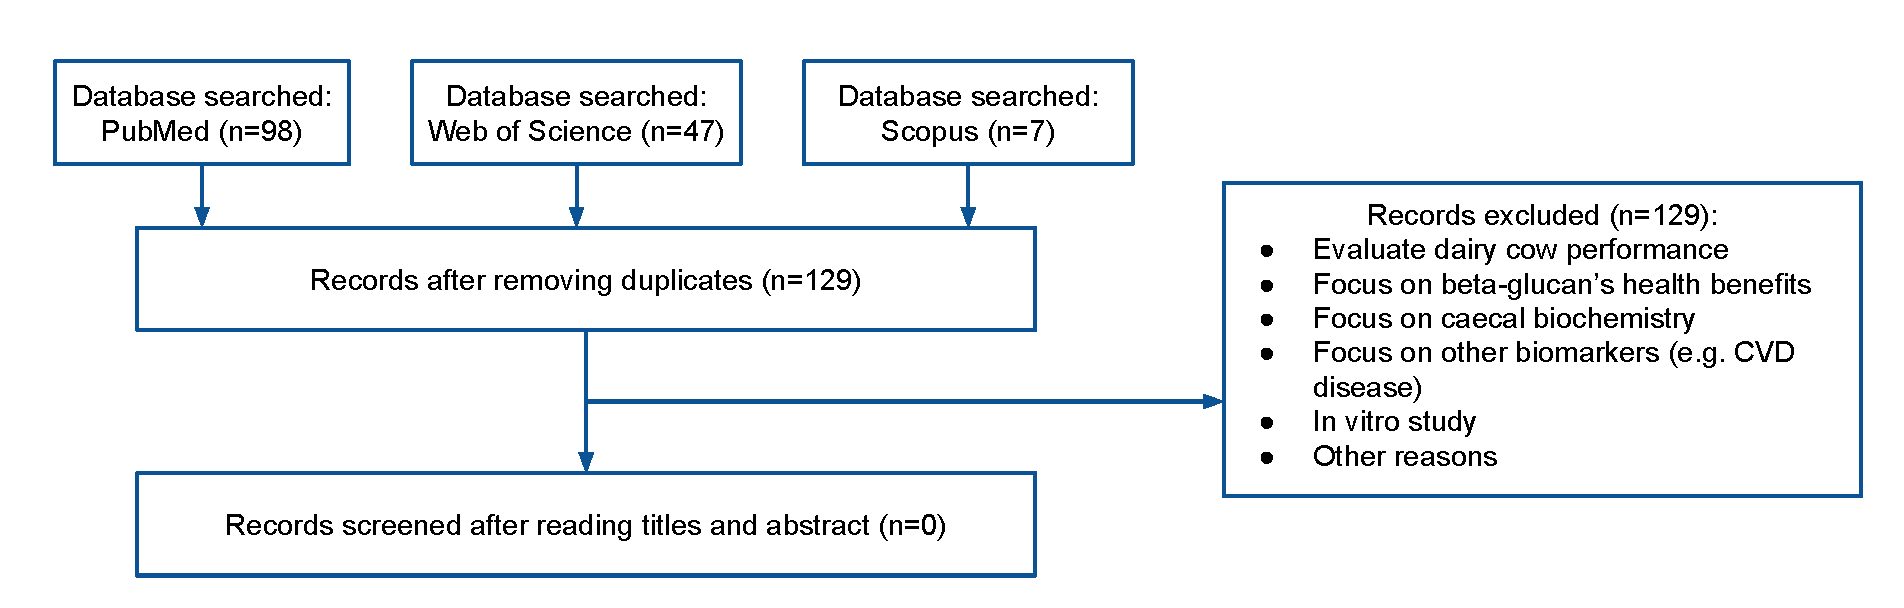
\includegraphics[width=\linewidth]{picture/barley_biomarker_review}
	\caption{Flow Chart of Literature Searching and Screening for Articles of WG Barley Intake Biomarkers}
	\label{fig:barleybiomarkerreview}
\end{figure}

\begin{figure}[h!]
	\centering
	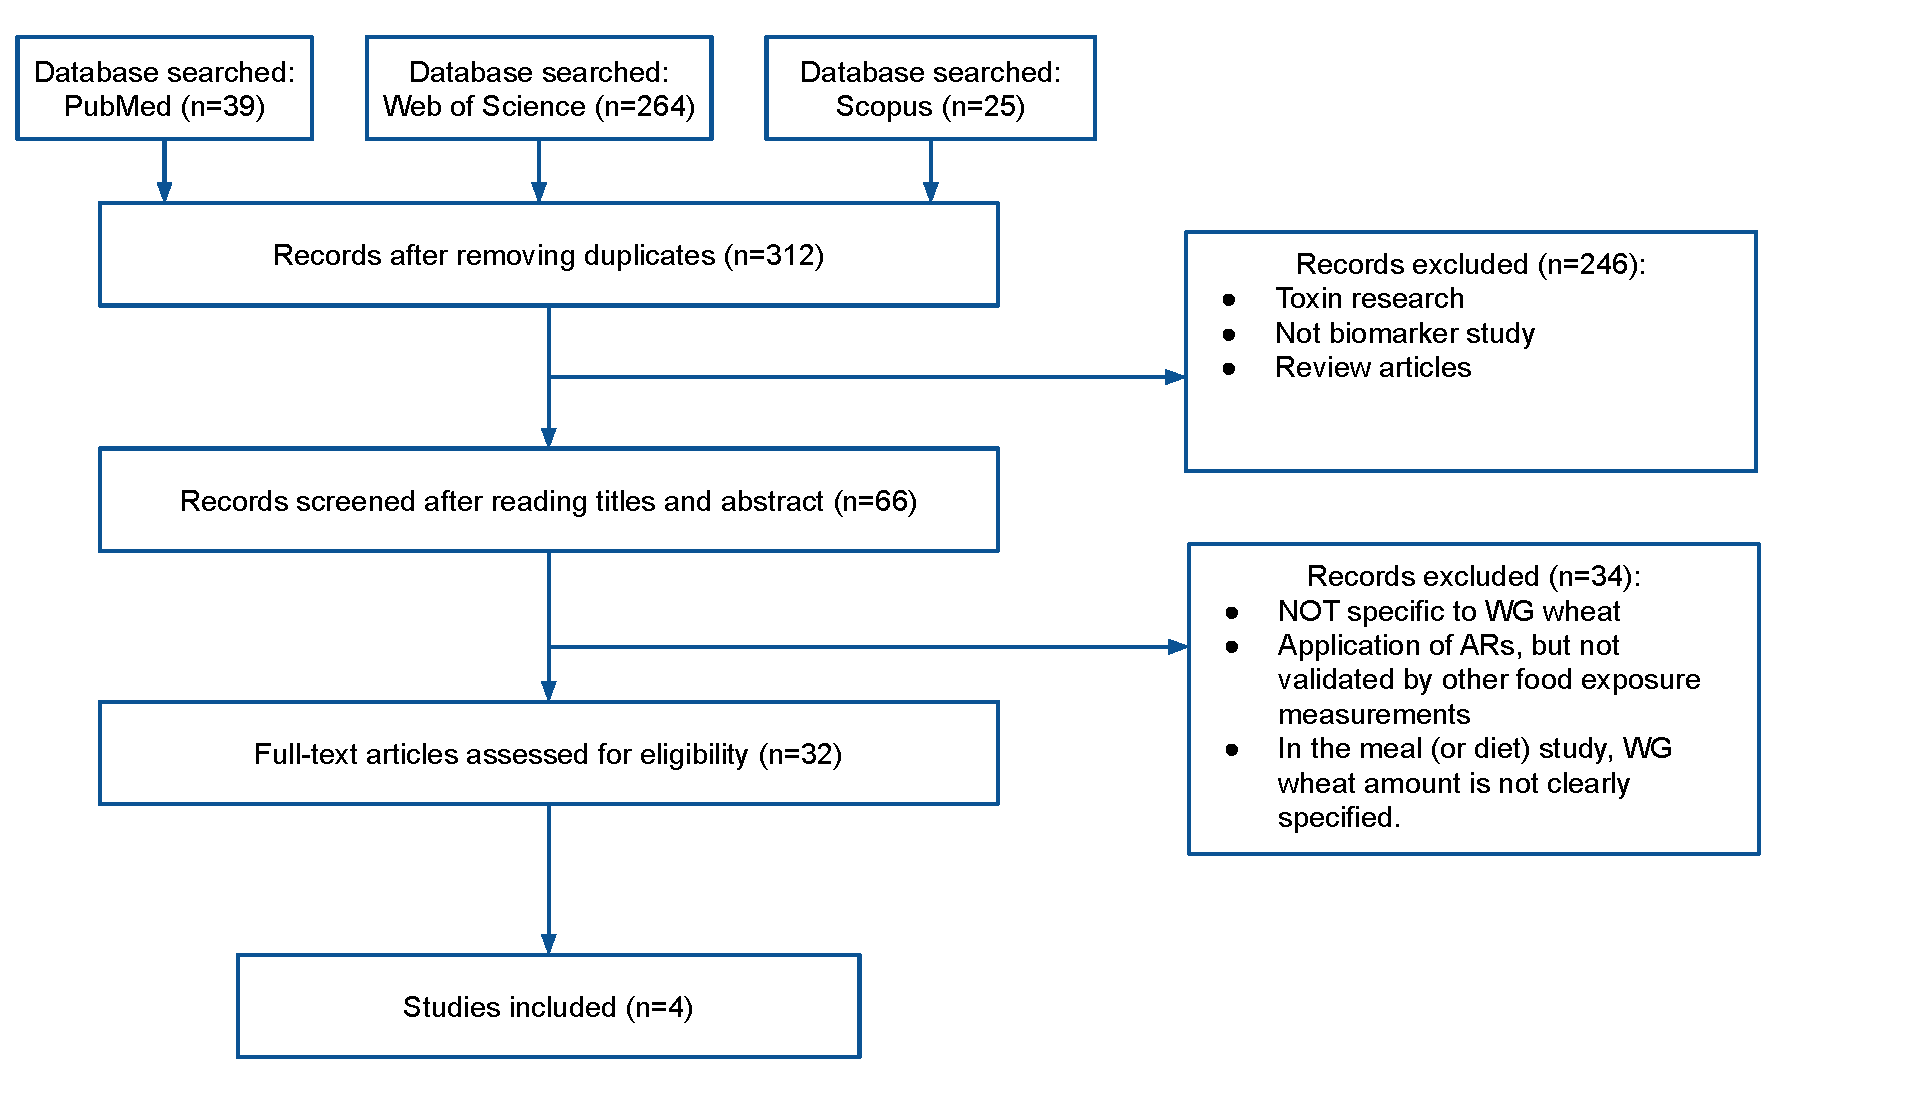
\includegraphics[width=\linewidth]{picture/wheat_biomarker_review}
	\caption{Flow Chart of Literature Searching and Screening for Articles of WG Wheat Intake Biomarkers}
	\label{fig:wheatbiomarkerreview}
\end{figure}

%%%%
{\centering
%\begin{landscape}
	\begin{table}[h!]
		\scalebox{0.7}{
			\begin{tabular}{|c|c|c|c|c|c|c|}
				%header
				\hline 
				\makecell{Dietary\\factor} &  \makecell{No.\\subjects} &\makecell{Study\\design} & \makecell{Sample\\type}  & \makecell{Analytical\\method} & \makecell{Candidate\\biomarker(s)} & Reference \\ 
				\hline
				%1st entry - betaine
				\makecell{Wheat bran,\\Wheat aleurone} & 14+13 & \makecell{randomized,\\ cross-over,\\ intervention} & \makecell{plasma}  & \makecell{LC-MS/MS\\ (Microbiology assay\\for folate)} & \makecell{betaine\\choline\\folate\\dimethylglycine (DMG)} & \cite{ISI:000350230300006} \\ 
				\hline
				
				%2nd entry - PREDIMED
				\makecell{None-bread,\\White bread,\\WG bread} & 155 & observation\footnote{dietary exposure measured from FFQ} & \makecell{\makecell{urine}}  & HPLC-qTOF-MS & \makecell{Benzoxazinoid-related metabolites\\(HHPAA, HBOA glycoside)\\ ARs-related metabolites\\ (DHPPA glucuronide, DHPPTA sulphate\\microbial-derived metabolites} & \cite{ISI:000348343300015} \\ 
				\hline
				
				%3rd entry
				%WGs\footnote{This study was conducted in US. WG wheat is the major WG source in US populations. However, these two metabolites were not specific to WG wheat. Because other cereals containing ARs could also be metabolized to these metabolites.} & 104 & observation (FFQ)& \makecell{spot\\urine}  & GC-MS & \makecell{ARs metabolites\\(DHBA, DHPPA)} & \cite{ISI:000303089700010} \\ 
				%\hline		
				%\hline 
				
				%4th entry
				\makecell{WGs\footnote{Several types of WGs were used (WG wheat, corn, oats, barley and rice), WG wheat made up around 65\% of the intervention}} & 266 & \makecell{randomized,\\ parallel-group,\\ intervention} & plasma & GC-MS & Total ARs & \cite{ISI:000298402100026} \\ 
				\hline 
				\end{tabular}}
		\caption{Reported markers distinguishing WG wheat intake, but NOT specific}
		\label{table:wheat_notspecific}
	\end{table}
}
%\end{landscape}}
